
\hskip-2cm
\resizebox{8cm}{!}{
    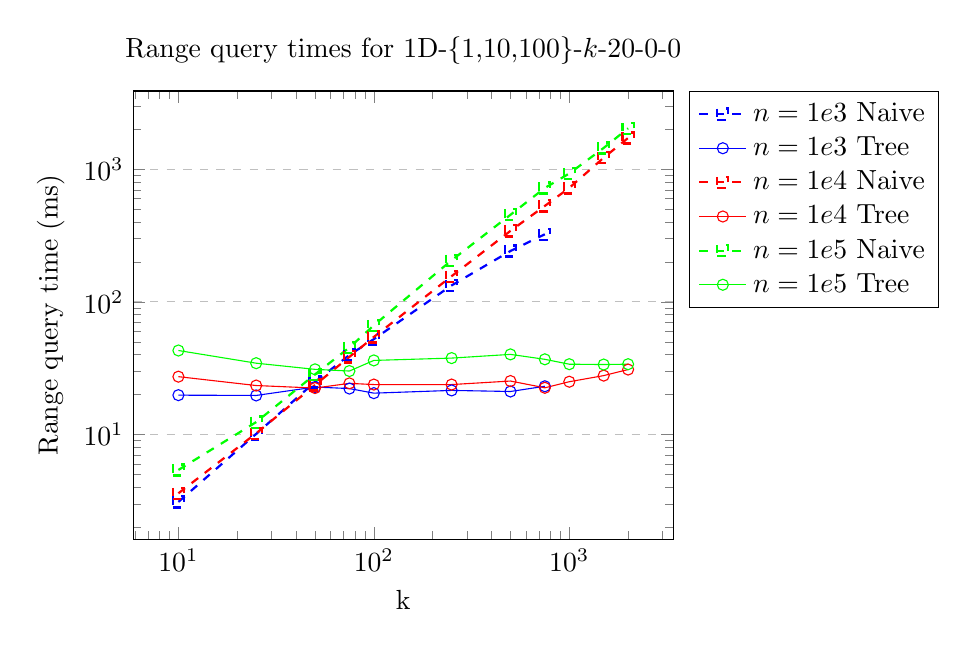
\begin{tikzpicture}
    \begin{axis}[
        title={Range query times for 1D-\{1,10,100\}-$k$-20-0-0},
        xmode=log,
        ymode=log,
        xlabel={k},
        ylabel={Range query time (ms)},
        legend pos=outer north east,
        ymajorgrids=true,
        grid style=dashed,
        legend cell align={left},
    ]
    \addplot[
        color=blue,
        mark=square,
        dashed, thick,
        ]
        coordinates {
            (10, 3.1)
            (25, 10.1)
            (50, 24.9)
            (75, 39.8)
            (100, 52.4)
            (250, 133.2)
            (500, 242.2)
            (750, 324.0)
        };
    \addlegendentry{$n=1e3$ Naive}
    \addplot[
        color=blue,
        mark=o,
        ]
        coordinates {
            (10, 19.8)
            (25, 19.7)
            (50, 22.8)
            (75, 22.2)
            (100, 20.5)
            (250, 21.5)
            (500, 21.1)
            (750, 23.1)
        };
    \addlegendentry{$n=1e3$ Tree}
    
    \addplot[
        color=red,
        mark=square,
        dashed, thick
        ]
        coordinates {
            (10, 3.6)
            (25, 10.2)
            (50, 23.6)
            (75, 38.5)
            (100, 54.4)
            (250, 156.4)
            (500, 343.5)
            (750, 530.0)
            (1000, 725.0)
            (1500, 1224.4)
            (2000, 1725.3)
        };
    \addlegendentry{$n=1e4$ Naive}
    \addplot[
        color=red,
        mark=o,
        ]
        coordinates {
        (10, 27.3)
        (25, 23.4)
        (50, 22.4)
        (75, 24.3)
        (100, 23.8)
        (250, 23.8)
        (500, 25.3)
        (750, 22.5)
        (1000, 25.0)
        (1500, 27.8)
        (2000, 30.9)
        };
    \addlegendentry{$n=1e4$ Tree}
    
    \addplot[
        color=green,
        mark=square,
        dashed, thick,
        ]
        coordinates {
            (10, 5.4)
            (25, 12.4)
            (50, 28.4)
            (75, 45.3)
            (100, 66.6)
            (250, 206.2)
            (500, 454.2)
            (750, 724.1)
            (1000, 931.0)
            (1500, 1450.9)
            (2000, 2040.4)
        };
    \addlegendentry{$n=1e5$ Naive}
    \addplot[
        color=green,
        mark=o,
        ]
        coordinates {
            (10, 43.0)
            (25, 34.5)
            (50, 31.0)
            (75, 30.1)
            (100, 36.2)
            (250, 37.7)
            (500, 40.2)
            (750, 36.9)
            (1000, 33.9)
            (1500, 33.7)
            (2000, 33.9)
        };
    \addlegendentry{$n=1e5$ Tree}
    \end{axis}
\end{tikzpicture}
}
\resizebox{8cm}{!}{
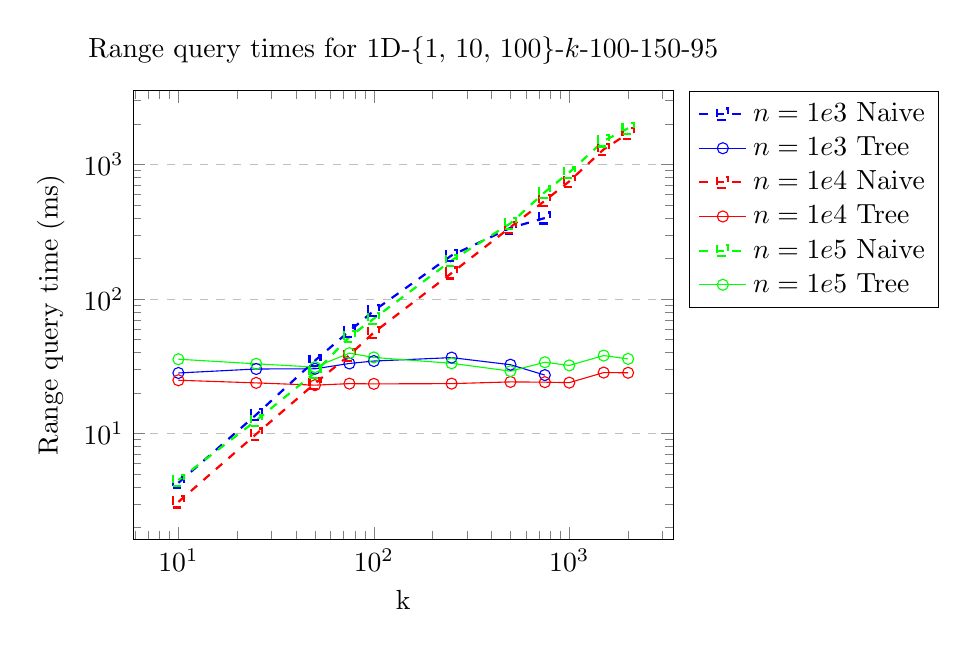
\begin{tikzpicture}
    \begin{axis}[
        title={Range query times for 1D-\{1, 10, 100\}-$k$-100-150-95 },
        xmode=log,
        ymode=log,
        xlabel={k},
        ylabel={Range query time (ms)},
        legend pos=outer north east,
        ymajorgrids=true,
        grid style=dashed,
        legend cell align={left},
    ]
    \addplot[
        color=blue,
        mark=square,
        dashed, thick,
        ]
        coordinates {
            (10, 4.3)
            (25, 13.8)
            (50, 34.9)
            (75, 57.8)
            (100, 81.9)
            (250, 211.2)
            (500, 338.5)
            (750, 400.6)
        };
    \addlegendentry{$n=1e3$ Naive}
    \addplot[
        color=blue,
        mark=o,
        ]
        coordinates {
            (10, 28.2)
            (25, 30.2)
            (50, 30.3)
            (75, 33.2)
            (100, 34.6)
            (250, 36.7)
            (500, 32.5)
            (750, 27.2)
        };
    \addlegendentry{$n=1e3$ Tree}
    
    \addplot[
        color=red,
        mark=square,
        dashed, thick
        ]
        coordinates {
            (10, 3.1)
            (25, 9.9)
            (50, 23.6)
            (75, 38.3)
            (100, 56.4)
            (250, 156.2)
            (500, 342.6)
            (750, 539.0)
            (1000, 751.2)
            (1500, 1298.7) 
(2000, 1704.1) 
        };
    \addlegendentry{$n=1e4$ Naive}
    \addplot[
        color=red,
        mark=o,
        ]
        coordinates {
            (10, 24.9)
            (25, 23.8)
            (50, 22.9)
            (75, 23.5)
            (100, 23.4)
            (250, 23.5)
            (500, 24.2)
            (750, 24.1)
            (1000, 23.9)
            (1500, 28.4)
(2000, 28.3)
        };
    \addlegendentry{$n=1e4$ Tree}
    
    \addplot[
        color=green,
        mark=square,
        dashed, thick,
        ]
        coordinates {
            (10, 4.5)
            (25, 12.5)
            (50, 28.4)
            (75, 52.4)
            (100, 71.5)
            (250, 193.9)
            (500, 365.6)
            (750, 624.7)
            (1000, 875.4)
            (1500, 1501.1)
(2000, 1862.5)
        };
    \addlegendentry{$n=1e5$ Naive}
    \addplot[
        color=green,
        mark=o,
        ]
        coordinates {
            (10, 35.7)
            (25, 33.0)
            (50, 31.2)
            (75, 39.6)
            (100, 36.8)
            (250, 33.3)
            (500, 29.1)
            (750, 33.9)
            (1000, 32.1)
            (1500, 38.0)
(2000, 35.9)
        };
    \addlegendentry{$n=1e5$ Tree}
    \end{axis}
    \end{tikzpicture}
}

% B1, B2, C1, C2
\hskip-2cm
\resizebox{8cm}{!}{
    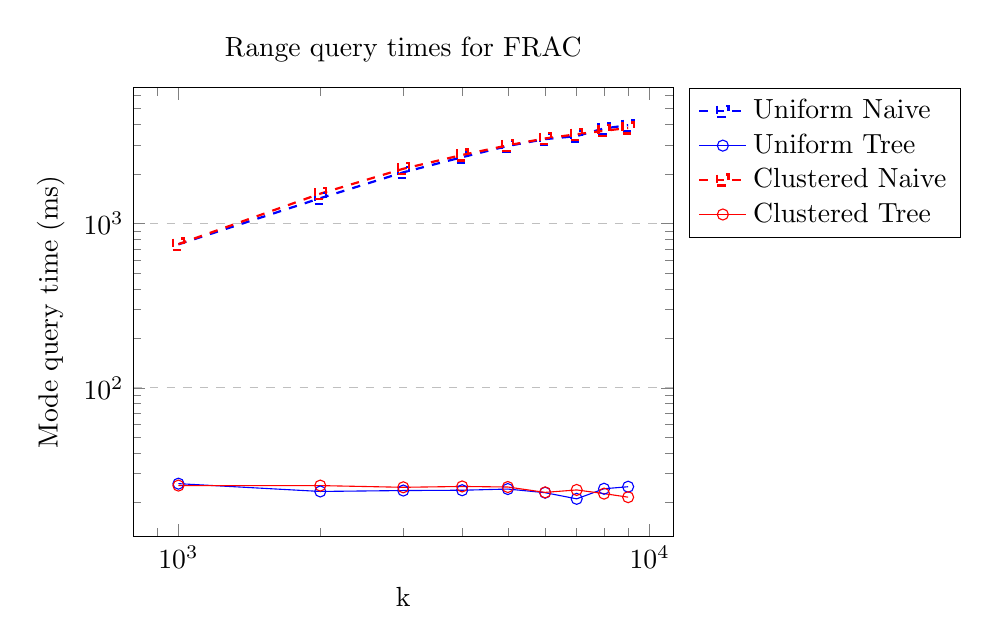
\begin{tikzpicture}
    \begin{axis}[
        title={Range query times for FRAC},
        xmode=log,
        ymode=log,
        xlabel={k},
        ylabel={Mode query time (ms)},
        legend pos=outer north east,
        ymajorgrids=true,
        grid style=dashed,
        legend cell align={left},
    ]
    \addplot[
        color=blue,
        mark=square,
        dashed, thick,
        ]
        coordinates {
            (1000, 746.1)
            (2000, 1423.7)
            (3000, 2046.1)
            (4000, 2529.4)
            (5000, 2960.1)
            (6000, 3258.7)
            (7000, 3399.4)
            (8000, 3785.1)
            (9000, 3958.8)
        };
    \addlegendentry{Uniform Naive}
    \addplot[
        color=blue,
        mark=o,
        ]
        coordinates {
            (1000, 26.1)
            (2000, 23.4)
            (3000, 23.7)
            (4000, 23.8)
            (5000, 24.2)
            (6000, 23.0)
            (7000, 21.1)
            (8000, 24.3)
            (9000, 25.0)
        };
    \addlegendentry{Uniform Tree}
    
    \addplot[
        color=red,
        mark=square,
        dashed, thick
        ]
        coordinates {
            (1000, 748.2)
            (2000, 1517.7)
            (3000, 2151.0)
            (4000, 2609.7)
            (5000, 2986.5)
            (6000, 3289.9)
            (7000, 3489.2)
            (8000, 3661.8)
            (9000, 3808.8)
        };
    \addlegendentry{Clustered Naive}
    \addplot[
        color=red,
        mark=o,
        ]
        coordinates {
            (1000, 25.4)
            (2000, 25.4)
            (3000, 24.8)
            (4000, 25.1)
            (5000, 24.9)
            (6000, 23.1)
            (7000, 23.9)
            (8000, 22.7)
            (9000, 21.6)
        };
    \addlegendentry{Clustered Tree}
    \end{axis}
    \end{tikzpicture}
}
\resizebox{8cm}{!}{
    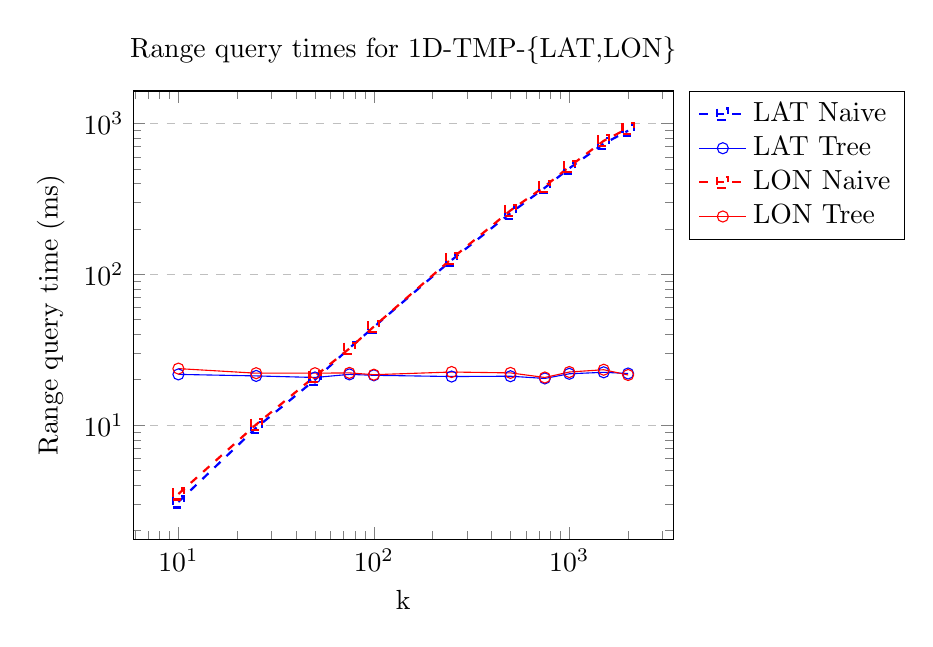
\begin{tikzpicture}
    \begin{axis}[
        title={Range query times for 1D-TMP-\{LAT,LON\}},
        xmode=log,
        ymode=log,
        xlabel={k},
        ylabel={Range query time (ms)},
        legend pos=outer north east,
        ymajorgrids=true,
        grid style=dashed,
        legend cell align={left},
    ]
    \addplot[
        color=blue,
        mark=square,
        dashed, thick,
        ]
        coordinates {
            (10, 3.1)
            (25, 9.6)
            (50, 20.0)
            (75, 32.4)
            (100, 44.7)
            (250, 124.1)
            (500, 254.2)
            (750, 374.5)
            (1000, 503.8)
            (1500, 733.0)
(2000, 894.4)
        };
    \addlegendentry{LAT Naive}
    \addplot[
        color=blue,
        mark=o,
        ]
        coordinates {
            (10, 21.7)
            (25, 21.2)
            (50, 20.7)
            (75, 21.7)
            (100, 21.4)
            (250, 21.0)
            (500, 21.1)
            (750, 20.4)
            (1000, 21.9)
            (1500, 22.4)
(2000, 22.0)
        };
    \addlegendentry{LAT Tree}
    
    \addplot[
        color=red,
        mark=square,
        dashed, thick
        ]
        coordinates {
            (10, 3.5)
            (25, 10.1)
            (50, 21.1)
            (75, 32.2)
            (100, 45.0)
            (250, 126.8)
            (500, 264.6)
            (750, 382.6)
            (1000, 516.3)
            (1500, 766.4)
(2000, 927.4)
        };
    \addlegendentry{LON Naive}
    \addplot[
        color=red,
        mark=o,
        ]
        coordinates {
            (10, 23.7)
            (25, 22.1)
            (50, 22.1)
            (75, 22.2)
            (100, 21.6)
            (250, 22.5)
            (500, 22.2)
            (750, 20.7)
            (1000, 22.5)
            (1500, 23.3)
(2000, 21.5)
        };
    \addlegendentry{LON Tree}
    \end{axis}
    \end{tikzpicture}
}

% All data
% \hskip-2cm
% \resizebox{8cm}{!}{
%     \begin{tikzpicture}
%     \begin{axis}[
%         title={Range query times for A1-A3},
%         xmode=log,
%         ymode=log,
%         xlabel={k},
%         ylabel={Range query time (ms)},
%         legend pos=outer north east,
%         ymajorgrids=true,
%         grid style=dashed,
%     ]
%     \addplot[
%         color=blue,
%         mark=square,
%         dashed, thick,
%         ]
%         coordinates {
%             (10, 3.1)
%             (25, 10.1)
%             (50, 24.9)
%             (75, 39.8)
%             (100, 52.4)
%             (250, 133.2)
%             (500, 242.2)
%             (750, 324.0)
%         };
%     \addlegendentry{A1 Naive}
%     \addplot[
%         color=blue,
%         mark=o,
%         ]
%         coordinates {
%             (10, 19.8)
%             (25, 19.7)
%             (50, 22.8)
%             (75, 22.2)
%             (100, 20.5)
%             (250, 21.5)
%             (500, 21.1)
%             (750, 23.1)
%         };
%     \addlegendentry{A1 Tree}
    
%     \addplot[
%         color=red,
%         mark=square,
%         dashed, thick
%         ]
%         coordinates {
%             (10, 3.6)
%             (25, 10.2)
%             (50, 23.6)
%             (75, 38.5)
%             (100, 54.4)
%             (250, 156.4)
%             (500, 343.5)
%             (750, 530.0)
%             (1000, 725.0)
%             (1500, 1224.4)
%             (2000, 1725.3)
%         };
%     \addlegendentry{A2 Naive}
%     \addplot[
%         color=red,
%         mark=o,
%         ]
%         coordinates {
%         (10, 27.3)
%         (25, 23.4)
%         (50, 22.4)
%         (75, 24.3)
%         (100, 23.8)
%         (250, 23.8)
%         (500, 25.3)
%         (750, 22.5)
%         (1000, 25.0)
%         (1500, 27.8)
%         (2000, 30.9)
%         };
%     \addlegendentry{A2 Tree}
    
%     \addplot[
%         color=green,
%         mark=square,
%         dashed, thick,
%         ]
%         coordinates {
%             (10, 5.4)
%             (25, 12.4)
%             (50, 28.4)
%             (75, 45.3)
%             (100, 66.6)
%             (250, 206.2)
%             (500, 454.2)
%             (750, 724.1)
%             (1000, 931.0)
%             (1500, 1450.9)
%             (2000, 2040.4)
%         };
%     \addlegendentry{A3 Naive}
%     \addplot[
%         color=green,
%         mark=o,
%         ]
%         coordinates {
%             (10, 43.0)
%             (25, 34.5)
%             (50, 31.0)
%             (75, 30.1)
%             (100, 36.2)
%             (250, 37.7)
%             (500, 40.2)
%             (750, 36.9)
%             (1000, 33.9)
%             (1500, 33.7)
%             (2000, 33.9)
%         };
%     \addlegendentry{A3 Tree}
%     \end{axis}
%     \end{tikzpicture}
% }
% \resizebox{8cm}{!}{
%     \begin{tikzpicture}
%     \begin{axis}[
%         title={Range query times for A4-A6},
%         xmode=log,
%         ymode=log,
%         xlabel={k},
%         ylabel={Range query time (ms)},
%         legend pos=outer north east,
%         ymajorgrids=true,
%         grid style=dashed,
%     ]
%     \addplot[
%         color=blue,
%         mark=square,
%         dashed, thick,
%         ]
%         coordinates {
%             (10, 3.5)
%             (25, 10.8)
%             (50, 24.8)
%             (75, 39.2)
%             (100, 58.2)
%             (250, 153.0)
%             (500, 290.8)
%             (750, 349.7)
%         };
%     \addlegendentry{A4 Naive}
%     \addplot[
%         color=blue,
%         mark=o,
%         ]
%         coordinates {
%             (10, 21.3)
%             (25, 21.7)
%             (50, 20.9)
%             (75, 21.6)
%             (100, 22.1)
%             (250, 26.6)
%             (500, 24.8)
%             (750, 24.4)
%         };
%     \addlegendentry{A4 Tree}
    
%     \addplot[
%         color=red,
%         mark=square,
%         dashed, thick
%         ]
%         coordinates {
%             (10, 3.3)
%             (25, 10.2)
%             (50, 23.6)
%             (75, 38.5)
%             (100, 54.9)
%             (250, 159.0)
%             (500, 345.1)
%             (750, 529.8)
%             (1000, 720.5)
%             (1500, 1271.0)
% (2000, 1713.8)
%         };
%     \addlegendentry{A5 Naive}
%     \addplot[
%         color=red,
%         mark=o,
%         ]
%         coordinates {
%             (10, 24.0)
%             (25, 23.0)
%             (50, 24.7)
%             (75, 22.4)
%             (100, 22.6)
%             (250, 24.1)
%             (500, 23.8)
%             (750, 23.0)
%             (1000, 22.7)
%             (1500, 28.3)
% (2000, 26.6)
%         };
%     \addlegendentry{A5 Tree}
    
%     \addplot[
%         color=green,
%         mark=square,
%         dashed, thick,
%         ]
%         coordinates {
%             (10, 4.5)
%             (25, 12.7)
%             (50, 28.3)
%             (75, 46.6)
%             (100, 66.3)
%             (250, 214.9)
%             (500, 445.1)
%             (750, 676.8)
%             (1000, 892.6)
%             (1500, 1448.5)
% (2000, 2074.2)
%         };
%     \addlegendentry{A6 Naive}
%     \addplot[
%         color=green,
%         mark=o,
%         ]
%         coordinates {
%             (10, 39.1)
%             (25, 35.2)
%             (50, 33.4)
%             (75, 30.9)
%             (100, 32.9)
%             (250, 37.8)
%             (500, 36.9)
%             (750, 32.5)
%             (1000, 33.1)
%             (1500, 33.5)
% (2000, 33.5)
%         };
%     \addlegendentry{A6 Tree}
%     \end{axis}
%     \end{tikzpicture}
% }

% % A7-A12
% \hskip-2cm
% \resizebox{8cm}{!}{
%     \begin{tikzpicture}
%     \begin{axis}[
%         title={Range query times for A7-A9},
%         xmode=log,
%         ymode=log,
%         xlabel={k},
%         ylabel={Range query time (ms)},
%         legend pos=outer north east,
%         ymajorgrids=true,
%         grid style=dashed,
%     ]
%     \addplot[
%         color=blue,
%         mark=square,
%         dashed, thick,
%         ]
%         coordinates {
%             (10, 3.8)
%             (25, 12.8)
%             (50, 32.4)
%             (75, 48.2)
%             (100, 65.0)
%             (250, 170.4)
%             (500, 301.1)
%             (750, 420.0)
%         };
%     \addlegendentry{A7 Naive}
%     \addplot[
%         color=blue,
%         mark=o,
%         ]
%         coordinates {
%             (10, 26.4)
%             (25, 27.8)
%             (50, 29.6)
%             (75, 26.7)
%             (100, 28.5)
%             (250, 31.4)
%             (500, 28.4)
%             (750, 34.8)
%         };
%     \addlegendentry{A7 Tree}
    
%     \addplot[
%         color=red,
%         mark=square,
%         dashed, thick
%         ]
%         coordinates {
%             (10, 3.4)
%             (25, 10.0)
%             (50, 23.5)
%             (75, 39.5)
%             (100, 55.6)
%             (250, 166.0)
%             (500, 348.6)
%             (750, 536.6)
%             (1000, 717.6)
%             (1500, 1317.7)
% (2000, 1691.2)
%         };
%     \addlegendentry{A8 Naive}
%     \addplot[
%         color=red,
%         mark=o,
%         ]
%         coordinates {
%             (10, 23.2)
%             (25, 21.9)
%             (50, 21.8)
%             (75, 24.2)
%             (100, 22.7)
%             (250, 25.3)
%             (500, 26.1)
%             (750, 24.3)
%             (1000, 23.0)
%             (1500, 27.4)
% (2000, 26.6)
%         };
%     \addlegendentry{A8 Tree}
    
%     \addplot[
%         color=green,
%         mark=square,
%         dashed, thick,
%         ]
%         coordinates {
%             (10, 4.6)
%             (25, 11.8)
%             (50, 27.3)
%             (75, 52.9)
%             (100, 68.9)
%             (250, 191.9)
%             (500, 368.1)
%             (750, 618.4)
%             (1000, 862.7)
%             (1500, 1474.6)
% (2000, 1880.3)
%         };
%     \addlegendentry{A9 Naive}
%     \addplot[
%         color=green,
%         mark=o,
%         ]
%         coordinates {
%             (10, 34.7)
%             (25, 31.7)
%             (50, 33.1)
%             (75, 33.7)
%             (100, 33.5)
%             (250, 33.4)
%             (500, 28.1)
%             (750, 31.2)
%             (1000, 31.5)
%             (1500, 39.5)
% (2000, 31.8)
%         };
%     \addlegendentry{A9 Tree}
%     \end{axis}
%     \end{tikzpicture}
% }
% \resizebox{8cm}{!}{
%     \begin{tikzpicture}
%     \begin{axis}[
%         title={Range query times for A10-A12},
%         xmode=log,
%         ymode=log,
%         xlabel={k},
%         ylabel={Range query time (ms)},
%         legend pos=outer north east,
%         ymajorgrids=true,
%         grid style=dashed,
%     ]
%     \addplot[
%         color=blue,
%         mark=square,
%         dashed, thick,
%         ]
%         coordinates {
%             (10, 4.3)
%             (25, 13.8)
%             (50, 34.9)
%             (75, 57.8)
%             (100, 81.9)
%             (250, 211.2)
%             (500, 338.5)
%             (750, 400.6)
%         };
%     \addlegendentry{A10 Naive}
%     \addplot[
%         color=blue,
%         mark=o,
%         ]
%         coordinates {
%             (10, 28.2)
%             (25, 30.2)
%             (50, 30.3)
%             (75, 33.2)
%             (100, 34.6)
%             (250, 36.7)
%             (500, 32.5)
%             (750, 27.2)
%         };
%     \addlegendentry{A10 Tree}
    
%     \addplot[
%         color=red,
%         mark=square,
%         dashed, thick
%         ]
%         coordinates {
%             (10, 3.1)
%             (25, 9.9)
%             (50, 23.6)
%             (75, 38.3)
%             (100, 56.4)
%             (250, 156.2)
%             (500, 342.6)
%             (750, 539.0)
%             (1000, 751.2)
%             (1500, 1298.7) 
% (2000, 1704.1) 
%         };
%     \addlegendentry{A11 Naive}
%     \addplot[
%         color=red,
%         mark=o,
%         ]
%         coordinates {
%             (10, 24.9)
%             (25, 23.8)
%             (50, 22.9)
%             (75, 23.5)
%             (100, 23.4)
%             (250, 23.5)
%             (500, 24.2)
%             (750, 24.1)
%             (1000, 23.9)
%             (1500, 28.4)
% (2000, 28.3)
%         };
%     \addlegendentry{A11 Tree}
    
%     \addplot[
%         color=green,
%         mark=square,
%         dashed, thick,
%         ]
%         coordinates {
%             (10, 4.5)
%             (25, 12.5)
%             (50, 28.4)
%             (75, 52.4)
%             (100, 71.5)
%             (250, 193.9)
%             (500, 365.6)
%             (750, 624.7)
%             (1000, 875.4)
%             (1500, 1501.1)
% (2000, 1862.5)
%         };
%     \addlegendentry{A12 Naive}
%     \addplot[
%         color=green,
%         mark=o,
%         ]
%         coordinates {
%             (10, 35.7)
%             (25, 33.0)
%             (50, 31.2)
%             (75, 39.6)
%             (100, 36.8)
%             (250, 33.3)
%             (500, 29.1)
%             (750, 33.9)
%             (1000, 32.1)
%             (1500, 38.0)
% (2000, 35.9)
%         };
%     \addlegendentry{A12 Tree}
%     \end{axis}
%     \end{tikzpicture}
% }

% % B1, B2, C1, C2
% \hskip-2cm
% \resizebox{8cm}{!}{
%     \begin{tikzpicture}
%     \begin{axis}[
%         title={Range query times for B1 and B2},
%         xmode=log,
%         ymode=log,
%         xlabel={k},
%         ylabel={Mode query time (ms)},
%         legend pos=outer north east,
%         ymajorgrids=true,
%         grid style=dashed,
%     ]
%     \addplot[
%         color=blue,
%         mark=square,
%         dashed, thick,
%         ]
%         coordinates {
%             (1000, 746.1)
%             (2000, 1423.7)
%             (3000, 2046.1)
%             (4000, 2529.4)
%             (5000, 2960.1)
%             (6000, 3258.7)
%             (7000, 3399.4)
%             (8000, 3785.1)
%             (9000, 3958.8)
%         };
%     \addlegendentry{B1 Naive}
%     \addplot[
%         color=blue,
%         mark=o,
%         ]
%         coordinates {
%             (1000, 26.1)
%             (2000, 23.4)
%             (3000, 23.7)
%             (4000, 23.8)
%             (5000, 24.2)
%             (6000, 23.0)
%             (7000, 21.1)
%             (8000, 24.3)
%             (9000, 25.0)
%         };
%     \addlegendentry{B1 Tree}
    
%     \addplot[
%         color=red,
%         mark=square,
%         dashed, thick
%         ]
%         coordinates {
%             (1000, 748.2)
%             (2000, 1517.7)
%             (3000, 2151.0)
%             (4000, 2609.7)
%             (5000, 2986.5)
%             (6000, 3289.9)
%             (7000, 3489.2)
%             (8000, 3661.8)
%             (9000, 3808.8)
%         };
%     \addlegendentry{B2 Naive}
%     \addplot[
%         color=red,
%         mark=o,
%         ]
%         coordinates {
%             (1000, 25.4)
%             (2000, 25.4)
%             (3000, 24.8)
%             (4000, 25.1)
%             (5000, 24.9)
%             (6000, 23.1)
%             (7000, 23.9)
%             (8000, 22.7)
%             (9000, 21.6)
%         };
%     \addlegendentry{B2 Tree}
%     \end{axis}
%     \end{tikzpicture}
% }
% \resizebox{8cm}{!}{
%     \begin{tikzpicture}
%     \begin{axis}[
%         title={Range query times for C1 and C2},
%         xmode=log,
%         ymode=log,
%         xlabel={k},
%         ylabel={Range query time (ms)},
%         legend pos=outer north east,
%         ymajorgrids=true,
%         grid style=dashed,
%     ]
%     \addplot[
%         color=blue,
%         mark=square,
%         dashed, thick,
%         ]
%         coordinates {
%             (10, 3.1)
%             (25, 9.6)
%             (50, 20.0)
%             (75, 32.4)
%             (100, 44.7)
%             (250, 124.1)
%             (500, 254.2)
%             (750, 374.5)
%             (1000, 503.8)
%             (1500, 733.0)
% (2000, 894.4)
%         };
%     \addlegendentry{C1 Naive}
%     \addplot[
%         color=blue,
%         mark=o,
%         ]
%         coordinates {
%             (10, 21.7)
%             (25, 21.2)
%             (50, 20.7)
%             (75, 21.7)
%             (100, 21.4)
%             (250, 21.0)
%             (500, 21.1)
%             (750, 20.4)
%             (1000, 21.9)
%             (1500, 22.4)
% (2000, 22.0)
%         };
%     \addlegendentry{C1 Tree}
    
%     \addplot[
%         color=red,
%         mark=square,
%         dashed, thick
%         ]
%         coordinates {
%             (10, 3.5)
%             (25, 10.1)
%             (50, 21.1)
%             (75, 32.2)
%             (100, 45.0)
%             (250, 126.8)
%             (500, 264.6)
%             (750, 382.6)
%             (1000, 516.3)
%             (1500, 766.4)
% (2000, 927.4)
%         };
%     \addlegendentry{C2 Naive}
%     \addplot[
%         color=red,
%         mark=o,
%         ]
%         coordinates {
%             (10, 23.7)
%             (25, 22.1)
%             (50, 22.1)
%             (75, 22.2)
%             (100, 21.6)
%             (250, 22.5)
%             (500, 22.2)
%             (750, 20.7)
%             (1000, 22.5)
%             (1500, 23.3)
% (2000, 21.5)
%         };
%     \addlegendentry{C2 Tree}
%     \end{axis}
%     \end{tikzpicture}
% }